\documentclass[12]{article}
\usepackage{chngcntr}

\usepackage{gensymb}
\usepackage{float}
\usepackage{float}
\usepackage{booktabs}
\usepackage{multirow}
\usepackage{amsmath}
\usepackage[utf8]{inputenc}
\usepackage[T1]{fontenc}
\usepackage{hyperref}
\usepackage{subcaption}
\usepackage{verbatim}
\usepackage{wrapfig}
\hypersetup{
    colorlinks,
    citecolor=black,
    filecolor=black,
    linkcolor=black,
    urlcolor=blue
}

\setlength{\oddsidemargin}{0.25 in}
\setlength{\evensidemargin}{-0.25 in}
\setlength{\topmargin}{-0.6 in}
\setlength{\textwidth}{18 cm}
\setlength{\textheight}{25 cm}
\setlength{\headsep}{0.75 in}
\setlength{\parindent}{0 in}
\setlength{\parskip}{0.1 in}
\usepackage{geometry}
\usepackage[final]{pdfpages}
\usepackage{textcomp}
\usepackage[table,xcdraw]{xcolor}
\counterwithin{figure}{subsection}
\usepackage{graphicx}
\usepackage[inkscapeformat=pdf,inkscapelatex=false]{svg}
\graphicspath{ {./Figs/} }

\begin{document}
\begin{titlepage}
\newcommand{\HRule}{\rule{\linewidth}{0.5mm}}
\setlength{\topmargin}{0 in}
\begin{center}
\begin{figure}[!h]
\centering

\includegraphics [width=0.3\textwidth]{eelogo.png}
\end{figure}

\vspace{10mm}
\Huge{MIDDLE EAST TECHNICAL UNIVERSITY}\\
\vspace{5mm}
{\LARGE ELECTRICAL \& ELECTRONICS ENGINEERING}\\

\HRule\\[0.4cm]
\textsc{\Large{EE464 - STATIC POWER CONVERSION II}}\\
\textsc{\Large{Hardware Project - Forward Converter \#1\\}}
\textsc{\Large{PowerLovers\\}}
\textsc{\Large{Final Report\\}}
\HRule\\[0.4cm]

\vspace{3mm}

\end{center}
\begin{minipage}{1\textwidth}
		\begin{flushleft}
			\large
			
			Emre Deniz  \textsc{Şenel - 2167237}\\
			Burak \textsc{Yalçın      - 2167534}\\
		
			
		\end{flushleft}
	\end{minipage}

\vspace{10mm}
\begin{center}
\large{24.06.2020}
\end{center}
\end{titlepage}

\tableofcontents
\newpage
\section{Introduction}

Static Power Conversion II, a self-defined course, offers numerous isolated and non-isolated converters, inverters and their applications. In Spring'20, the theoretical background that have been acquired is to be turned into a hardware implementation of the combined knowledge all together. However, due to the pandemic, it is not possible to introduce a product but present a detailed design with software supports and PCB design. In this report, forward converter design of group Powerlovers will be introduced. Background information with objectives will take place. Then, all the steps of the projects, tests, design procedures and simulation results will be exhibited. We strongly believe, this project helped us understand the concepts we learnt in the lectures, and we had a chance to see beyond the horizons.
\counterwithin{figure}{section}
\section{Problem Definition, Objectives and Bonus Points}

In the project, we are to do a forward converter design with specific properties.


\begin{table}[H]
\centering
\caption{Parameters of the project}
\label{tab:project_spec}
\resizebox{10 cm  }{!}{%
\begin{tabular}{|c|c|}
\hline
Minimum Input Voltage (V)             & \textbf{24} \\ \hline
Maximum Input Voltage (V)             & \textbf{48} \\ \hline
Output Voltage (V)                    & \textbf{15} \\ \hline
Output Power (W)                      & \textbf{48} \\ \hline
Output Volt. Peak-to-Peak Ripple (\%) & \textbf{2}  \\ \hline
Line Regulation (\%)                  & \textbf{2}  \\ \hline
Load Regulation (\%)                  & \textbf{2}  \\ \hline

\end{tabular}}
\end{table}

Some of the points and objectives can be itemized as:

\begin{itemize}
    \item Closed loop is a must and we are not allowed to use digital controllers
    \item PCB design of the converter will be presented.
    \item Bill of material will be presented
    \item Closed loop compansator design with bode-plot is a \textbf{bonus}
    \item We are to do thermal design and efficiency analysis of the project
\end{itemize}

We have mentioned couple of specifications of the project. Our goal was to accomplish the main specifications and add as much as bonus we can. 

In the next section we are introduce a forward converter.

\newpage
\counterwithin{figure}{subsection}
\section{Forward Converter}
\subsection{General Structure}

Forward converter is basically derived from the buck converter. We are going to observe the relationship in the derivation phase. Forward converter is isolated as we know, and it uses transformer as its regular use. Transformer transfers the power to the secondary side and it does not store energy in between. In forward converter, it is important to take the magnetizing current into account.

In Figure \ref{ForwardTopology}, the forward converter topology can be observed. This is the most simple model.

\begin{center}
\begin{figure}[H]
\centering
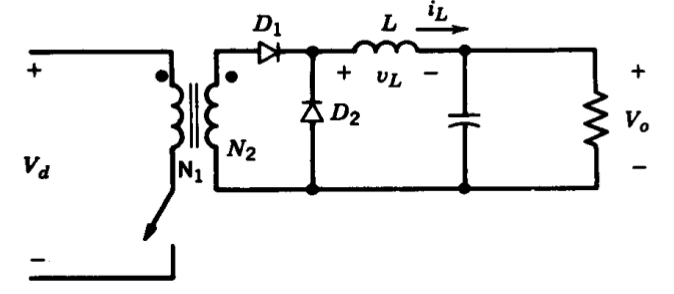
\includegraphics [width= 12 cm ]{forward.png}
\caption{Forward Converter Topology}
\label{ForwardTopology}
\end{figure}
\end{center}

Assume the transformer is ideal for now to obtain the transfer function of the topology. \\During the ON state of the switch, $D_{1}$ is conducting and $D_{2}$ is reverse biased. Therefore, the inductor voltage can be written down as $$V_{L} = \frac{N_2}{N_1}V_{d} - V_{o}$$

Let us examine now the OFF state of the switch. $D_{1}$ is now reverse biased on $D_{2}$ forms a free-wheeling path for the inductor. Load is fed by the stored energy in the inductor and the capacitor. Inductor voltage is easy to obtain and is as follows.$$V_{L} = - V_{o}$$

Discussion so far end with applying the voltage-seconds rule for the inductor and this yields the transfer function of the forward converter topology as 
\begin{equation}
    \frac{V_o}{V_d} = \frac{N_2}{N_1}D
\end{equation}
However, a question might arise rightfully at this point: how does this topology deal with the magnetizing current? During the OFF state, $L_m$ has no path to discharge and it seems to be charged again and again during ON state. This situation ends up saturating the core and threatens the proper operation of the converter. \\
A variety of solutions for this problem are available. A snubber circuitry connected in parallel to the primary winding, a two switch topology are among them. A more practical and wide-spread application ,however, is adding a third reset winding. The resultant topology can be seen in Figure \ref{PracticalForward}.

\begin{center}
\begin{figure}[H]
\centering
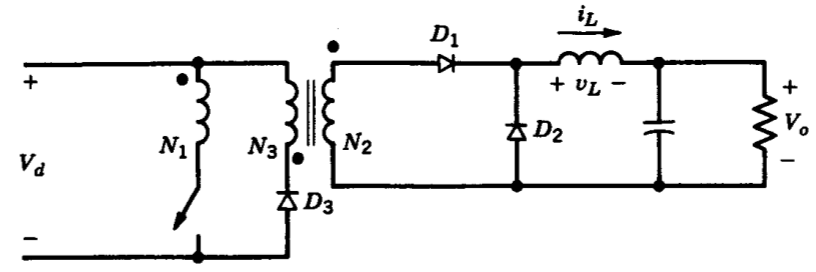
\includegraphics [width= 12 cm ]{practical_forward.png}
\caption{Practical Forward Converter Topology}
\label{PracticalForward}
\end{figure}
\end{center}

In this topology, the third winding namely $N_3$ is in use in order to reset the winding so that the core does not saturate. As its nature opposes, the forward converter has limitations itself. One and the most important thing is that $D_max$ namely maximum duty cycle is limited to the following equation

\begin{equation}
    D_{max} = \dfrac{1}{1 + N_3/N_1}
\end{equation}

In most of the cases, $N_1 = N_3$ is taken to simplify the structure and the organization. We followed the same approach in our solutions.

\section{Design of the Forward Converter}
\subsection{System Level Design}

The most important element in isolated power supplies is the transformer. Without knowing the transformer properties, it is not possible to move on with the simulations. Hence, the design process is now orderly. Output inductor and capacitor can also be chosen by theoretical knowledge.

Although it is possible to have a "pre-simulation" idea on the voltage stresses or current carrying capabilities for the semiconductor devices in the topology, it is safer to choose them in the guidance of the simulation results. Some of the non-idealities will also be involved in the simulations as well, allowing us to make more accurate assumptions about component selection. 

In this part, we need to look at general specifications of the forward converter. Our customer, from Habelsan, asked us to  satisfy these specifications:

\begin{itemize}
    \item Input voltage rate: $24V-48V$
    \item Output voltage: $15V$
    \item Output power: $48W$
    \item Output voltage ripple: $2\%$, maximum
    \item Line and Load regulations: $2\%$, maximum
\end{itemize}

Firstly, we need to look at input-output voltage relationship of the forward converter. Ratio between the two is derived in the previous parts as:

\begin{equation}
    \frac{V_o}{V_d} = \frac{N_2}{N_1}D
\end{equation}

Output current's average value is $\frac{48W}{15V} = 3.2A$. As mentioned before, demagnetization of the core in the forward converter is important. Among different techniques,it is decided to use a reset winding. Turn number of the reset winding is chosen to be equal to that of the primary winding, conventionally and we will stick to that convention as well. This situation puts a restriction on the duty cycle to ensure proper demagnetization of the core.Duty cycle for the operation should be $D < 0.5$.

\textbf{Turns Ratio \& Duty Cycle}

In the project, required voltage transfer ratios are 48V to 15V, and 24V to 15V. It is important to take into account that the limit of duty cycle is $D_{max} = 0.5$, and it is very crucial to reset all the core.

Using the input output equation and duty cycle restrictions, we choose the turn ratio between first and secondary winding as:

$$\frac{N_2}{N_1} = 2$$


Using these ratio, it is now easy to find required duty ratios. For 48V input,

$$D = \frac{48}{15} = 2 \implies D_{min} = 0.156$$

and For 24V input,

$$D = \frac{24}{15} = 2 \implies D_{max} = 0.3125$$

As can be seen, the duty cycle ratios obey the restrictions and they also allow a margin to compensate for the non-idealities.

\textbf{Frequency}

As switching frequency of the MOSFET, it is important to note that higher frequencies increases the switching losses. Also, at high frequencies, skin depth of the cable decreases dramatically. Moreover, it is also needed to be pointed that at higher frequencies hysteresis losses increase in the core. Therefore, we decided to keep our frequency less than 30kHz, $f < 30kHz$

Secondly, as frequency decreases, the amount of ripple at the output increases due to longer switching periods. Furthermore, it is important to keep the frequency at inaudible range so that the converter is not noisy. We decided that frequency should be higher than 20kHz, $f > 20kHz$.

Combining these two
$$20 kHz < f < 30kHz$$
In the simulations, we decided as the best frequency would be 25kHz. Therefore, for our forward converter the frequency is $f = 25kHz$


\subsection{Transformer Design}
In the forward converter topology, it is important to realize the fact that transformer is introduced in order to transfer the power from primary to secondary. For this reason, we do not need any air gap in our transformer design. Moreover, a transformer with high inductance will allow us to operate in low magnetizing current levels due to high impedance of the inductor. When we combine these, we can start our calculations.

The first approach is to calculate $WaAc$, it shows the power handling capacity of our transformer. Its formula is as follows:

\begin{equation}
    W_a A_c = \dfrac{P_o D_{cma}}{K_t B_{max} f}
\end{equation}

Here $P_o = 48W$, power out in watts, $D_{cma} = 500 \; cir/mils.amp$, is current density, $K_t = 0.0005$, topology constant given for forward converter. $B_{max} = 2500 G$, maximum flux density in gauss and $f=25kHz$ is the frequency. 

When we calculate the result

$$ W_a A_c = 0.768 \; cm^4$$

Now, using the magnetics' available cores offered for power handling capacities, we are going to choose a proper core. We chose an R material E shaped core, it is high in inductance and low in loss. It is very proper for this application.

The core link: \href{https://www.mag-inc.com/Media/Magnetics/Datasheets/0R43515EC.pdf}{Core}

Now it is important to choose turn number for primary side. The secondary and third windings depend on the primary side. We are going to apply following approach:

\begin{equation}
    N_p = \dfrac{V_p 10^8}{4BA_c f}
\end{equation}

We choose following parameters for this application: $V_p = 48V$, $B = 0.25 T $, $A_c = 0.87 cm^2$ it given in the datasheet of the core and $f=25kHz$. The result is:

$$N_p = 22 \; turn$$

Naturally, we have $N_1 = 22, N_2 = 44, N_3 = 22$ due to our selection.


The turns number for windings are determined as 
\begin{itemize}
    \item Primary winding, $n_1 = \textbf{22 turns}$
    \item Reset winding, $n_3 = \textbf{22 turns}$
    \item Secondary winding, $n_2 = \textbf{44 turns}$
\end{itemize}

Now, it is very important to take magnetizing inductance into account. In the datasheet we can easily see that the AL value is given as $AL = 2667 nH/T^2$. As we decided our turn number is 22, we can easily calculate the magnetizing inductance as:

$$ L_m = 22^2 * 2667 * 10^{-9} = 1.3 mH$$

This is a great value becuase a low magnetizing inductance will increase the magnetizing current at the primary side, as a result we would need a higher current capability. However, 1.3mH is a legitimate value. If we calculate the magnetizing current at operating frequency:

$$ I_m = \dfrac{V}{Z} = 0.235 A $$


\subsection{Cable Selection}


In practical cases maximum fill factor achievable is stated at 50\%. We need to take these two parameters into account.

Moreover, it is important to notice that, the input current at the maximum operation is $I_{in} = 2A$ and $I_m = 0.235A$, as overall we need minimum of $I_1 = 2.3A$ at the primary side. At the secondary side we are going to have a maximum of $I_o = 3.2A$, we have to take these into account. 

Using a simple approach $1 mm^2$ of cable can carry $4A$, and considering skin depth. We have chosen to use AWG22 cable. It's area is $0.327 mm^2$ and it can carry a current up to $1.3A$. Also, it's maximum skin depth is applicable up to $42kHz$, that is to say since our operating frequency is $25kHz$, this cable is proper to use. Considering margins, we are going to choose needed parallel cable amount.

In the output we need 2 parallel cables, and at the output we need 3 parallel cables.

Now, it is important to have a look at the fill factor. It is very crucial to have a fill factor around $50\%$ so that our transformer is realizable. 

If we calculate the cable areas:

$$A_{cable} = 0.326*22 + 0.326*22 + 0.326*44 = 71.9 mm^2$$

If we check our core's window area, we can see that it is:

$$A_{window} = 9.8*8*2 = 156.8 mm^2 $$

So the fill factor of our transformer is:

$$k = \dfrac{61.1}{156.8} = 46\%$$

This fill factor is applicable and not an overdesign. Therefore, the cable selections are proper. We have a legitimate fill factor, we have 100\% skin depth, and we have margins so that there is no burnout. In the next step we are going to cover the capacitor and inductor.


\subsection{Inductor and Capacitor Design}

To design the inductor, we are focus on the maximum ripple current allowed. In the specifications, it is not determined, so we are going to have 20\% maximum ripple current so that our output current would be out of harmonics and the filtering capacitor would be smaller.

At the ON period, the inductor is charging, and using the voltage among the terminals we can find the ripple current value.

$$ \Delta I = \frac{1}{L} \int_{0}^{DT_s} V_L dt < \dfrac{3.2A}{5} $$

$$ \Delta I = \frac{1}{L} \int_{0}^{DT_s} (V_s \frac{N_2}{N_1} - V_o) dt < 0.64A$$

$$ 0.62mH < L$$

Also, it is very important to take rated current into account. The minimum rated current that inductor can carry must be minimum of $3.2A + 0.65A \approx 3.8A$

Using digikey website, we chose a proper inductor. It is important to have a small inductor in order to decrease the size and the weight.

Inductor Link: \href{https://www.digikey.com/product-detail/en/bourns-inc/2300LL-681-H-RC/2300LL-681-H-RC-ND/725890}{Inductor}

Capacitor design is depending on the inductor design. As we know, we have to limit the ripple value of the output voltage. Also, the current that is flowing through the output is equal to the inductor current. We need to follow the following approach.

\begin{equation}
    \Delta V = \dfrac{\Delta Q}{C}
\end{equation}

\begin{equation}
    \Delta Q = \Delta I_L * \dfrac{T_s}{8}
\end{equation}

Here, we are using buck converter capacitor design approach. They are same in the application:

$$ \Delta V = 0.3V > \dfrac{DT_s^2 (V_s \dfrac{N_2}{N_1} - V_o) }{8LC}$$

$$ C > 28 \micro F$$

Also, apparently the rated voltage of the capacitor should be higher than the rated voltage of the output, for that reason $C_{v,rated} > 15V$

Capacitor Link: \href{https://product.tdk.com/info/en/documents/chara_sheet/C3216JB1E336M160AC.pdf}{Capacitor}

ESR value of the capacitor is: 


\subsection{Switch and Diode Design}

In these voltage levels and frequency levels it is proper to use MOSFET due to their fast recovery. It is also easy to implement a MOSFET into a converter. While designing the MOSFET, it is very important not to exceed its rated voltage and current values.

In the simulations with idealities, we came up with the values that:

\begin{itemize}
    \item Switches' stress have their maximum values for input of 48V naturally. We can say that switches must be endurable minimum of 100V rated reverse voltage and 10A forward voltage.
    \item Switches must be proper to operate at 25kHz range, reverse recovery times should be appropriate.
\end{itemize}

The MOSFET Link: \href{https://www.digikey.com/product-detail/en/on-semiconductor/FDMS86255/FDMS86255TR-ND/4555505}{MOSFET}



Silicon diodes are proper because they are cheap in cost and they have proper operation for this implementation range. 

In the simulations with idealities, we came up with the values that:

\begin{itemize}
    \item Diode' stress have their maximum values for input of 48V naturally. We can say that switches must be endurable minimum of 100V rated reverse voltage and 4A forward voltage.
    \item Diode must be proper to operate at 25kHz range, reverse recovery times should be appropriate.
\end{itemize}

Results of simulations will be introduced at next part.

\subsection{Feedback Controller Circuitry}

To keep the voltage constant at 15V and to satisfy the line/load regulations, an analog controller IC is to be used. A very popular PWM controller IC for power supplies, \textbf{TL494} by \emph{Texas Instruments} is chosen. Additional features comes with it makes it a favorable choice and in this section, some of them that we implemented in our design are to be presented.

To power up the module, a DC-DC converter is used. 


TL494 is able to drive two switches together, but only one of the outputs is to be used in our project. Soft starting and current limiting features are to be adapted to our application, though. Additional circuitry for them can be found in the application notes regarding TL494. 

To ensure electrical isolation between input and output sections of the converter, an optocoupler is to be used to drive the switching element. Our choice for this element is \textbf{TLP250} by \emph{Toshiba}. It is a familiar IC for us, since it is used previously on the hardware project of EE463.
\newpage
\section{Ideal Simulations}
\subsection{Simulation Results}
Below in the Figure \ref{simulation}, the simulation model schematic can be seen.

\begin{center}
\begin{figure}[H]
\centering
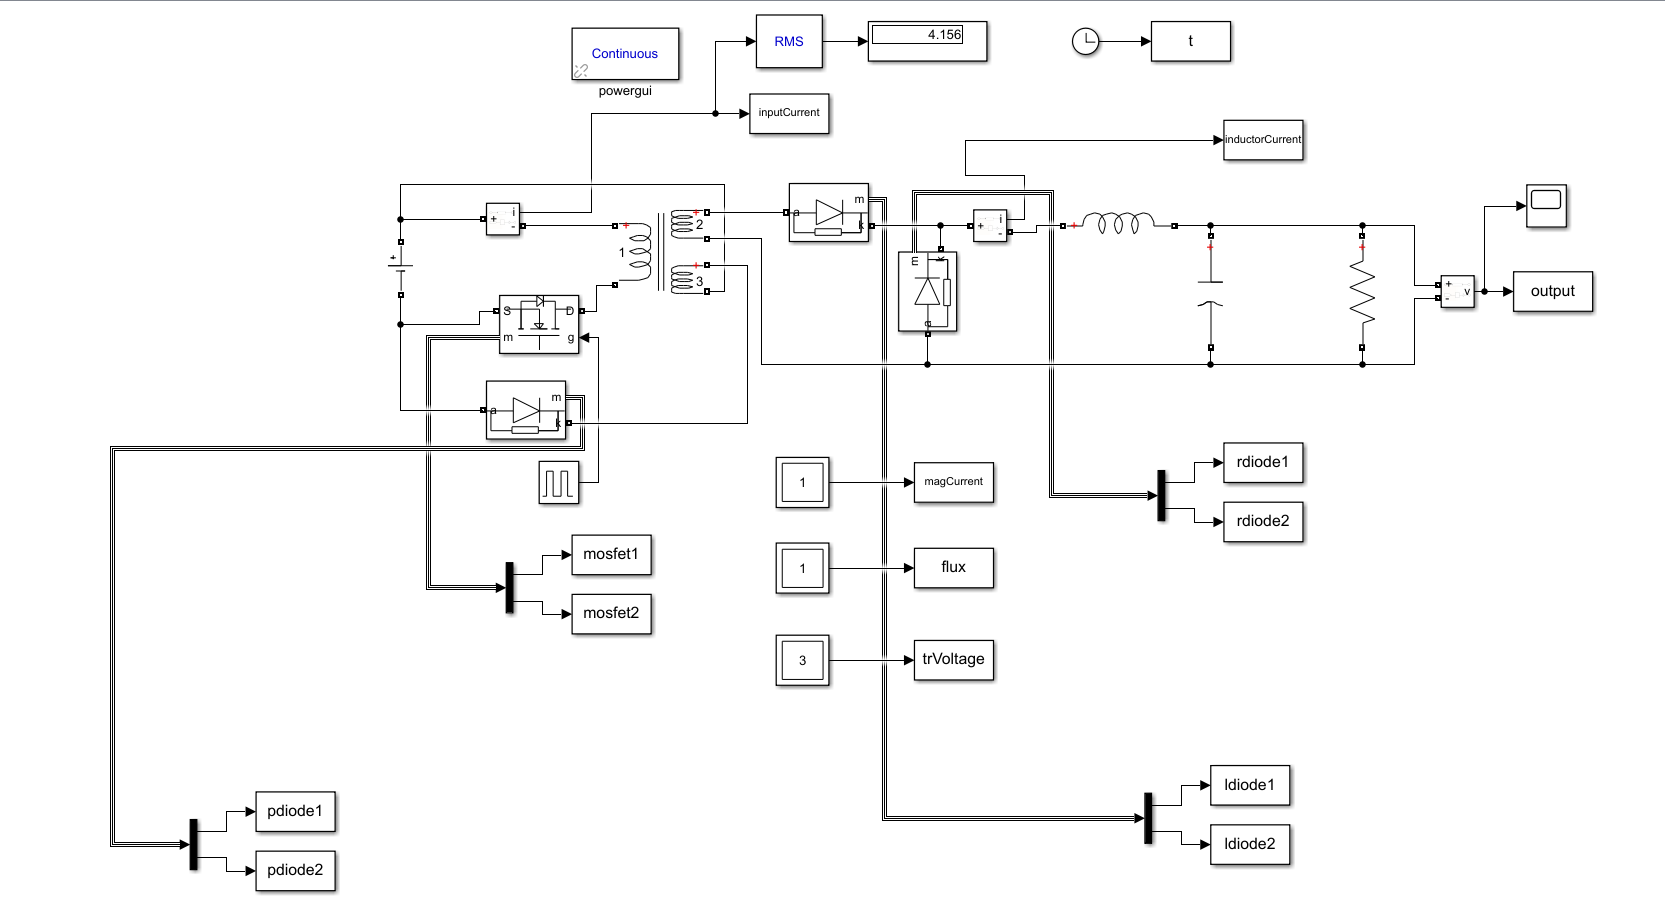
\includegraphics [width=15 cm]{simulation.png}
\caption{Simulation model}
\label{simulation}
\end{figure}
\end{center}

First, we simulated the ideal models in order to see the overall system operation. It is open-loop operation simulation and we would like to validate the duty cycles, operation principle and validity of our selections.

\begin{center}
\begin{figure}[H]
\centering
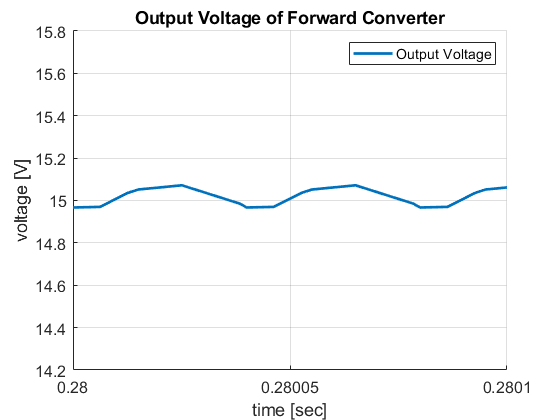
\includegraphics [width=12 cm, height= 8 cm]{output_voltage.png}
\caption{Output waveform of the forward converter under 48V operation}
\label{Output48}
\end{figure}
\end{center}

\begin{figure}[H]
\centering
\begin{subfigure}{7 cm}
  \centering
  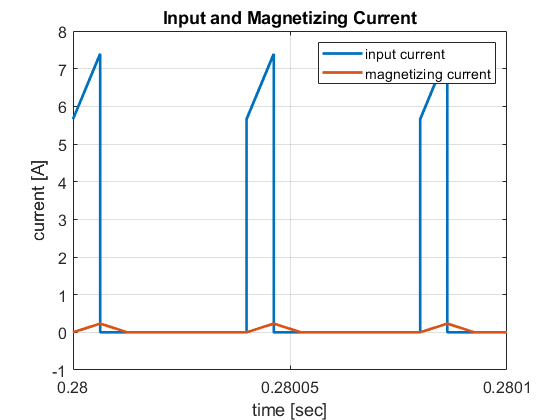
\includegraphics[width=7 cm]{input_current}
  \caption{Input and Magnetizing Current}
  \label{fig:input_current_48}
\end{subfigure}%
\begin{subfigure}{7 cm}
  \centering
  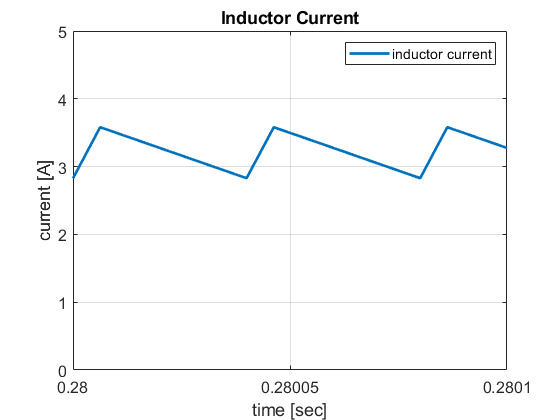
\includegraphics[width=7 cm]{inductor_current}
  \caption{Inductor Current}
  \label{fig:inductor_current_48}
\end{subfigure}
\caption{Forward converter input and inductor current under 48V input operation}
\label{fig:current_48}
\end{figure}


\begin{center}
\begin{figure}[H]
\centering
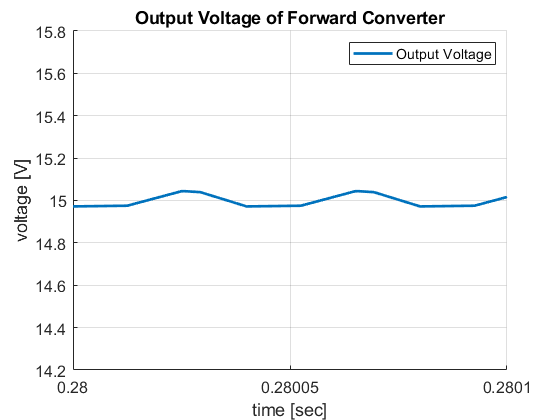
\includegraphics [width=12 cm, height= 8 cm]{output_voltage_24.png}
\caption{Output waveform of the forward converter under 24V operation}
\label{Output24}
\end{figure}
\end{center}

\begin{figure}[H]
\centering
\begin{subfigure}{7 cm}
  \centering
  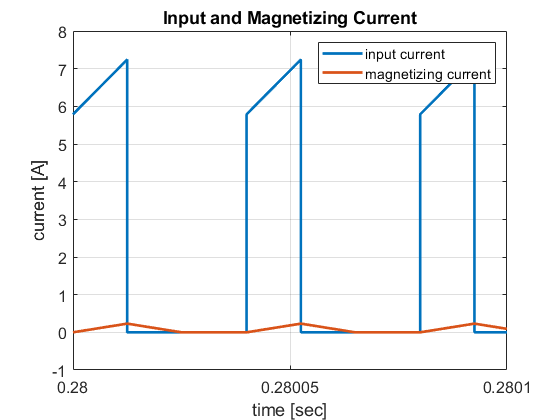
\includegraphics[width=7 cm]{input_current_24}
  \caption{Input and Magnetizing Current}
  \label{fig:input_current_24}
\end{subfigure}%
\begin{subfigure}{7 cm}
  \centering
  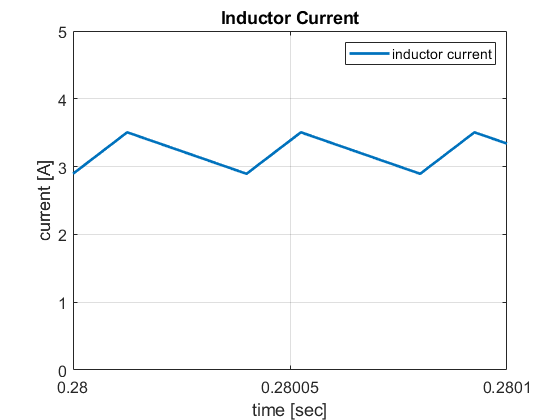
\includegraphics[width=7 cm]{inductor_current_24}
  \caption{Inductor Current}
  \label{fig:inductor_current_24}
\end{subfigure}
\caption{Forward converter input and inductor current under 24V input operation}
\label{fig:current_24}
\end{figure}


As we can see from the Fig. \ref{Output24} and \ref{Output48} the output ripple is below $2\%$. The operation is stable and the duty cycles are as expected. However, when non-idealities are presented the duty cycle values will be re-calculated in order to compansate the voltage drops of losses and diodes etc. 

Also, from the Fig. \ref{fig:current_24} and \ref{fig:current_48}, we can observe the magnetizing current is as expected around $0.3A$ and the inductor ripple is around $0.6A$ for both operations. These results show that our calculations are valid. Now we are going to add non-idealities of the circuit.








\section{Non-idealities of Forward Converter}

\subsection{Adding the Non-idealities and Their Solutions}

Firstly, we added the loss components of the MOSFET and the diodes. As we can see from the datasheet, MOSFET has $R_{ds,ON} = 12.4 m\ohm$, this value is added to the MOSFET. Then, the forward voltage values of the diodes are added to the software $V_f = 0.7V$ in our operation topology. After adding these, $R_{d,ON} = 1 m\ohm$ added for the diodes representing the losses on the selected diodes.

Series resistance of the inductor is given as maximum of $R_{max} = 0.113 \ohm$ for convenience we took this value as $0.6 \ohm$ to obtain an average operation range. Also, using the datasheet of the capacitor, we found out that the ESR value of the capacitor is around $3 m\ohm$. This is a low value, because the capacitor is a seramic capacitor and it has very low ESR operation.

Next step was to add the leakage inductances of the transformer, we have taken the leakage inductance as 1\% of the magnetizing inductance and introduced the leakage inductance as $13 \micro H$ to the primary side of the transformer.

Then it is very crucial to notice that the stored energy in the leakage inductance needs a way to decharge itself. For this very reason it is very important to design a snubber circuit around the MOSFET in order to block burnouts and have a smooth operation. We have decided to move on with a RC Snubber.

\begin{wrapfigure}{r}{0.5\textwidth}
  \vspace{-10pt}
  \begin{center}
    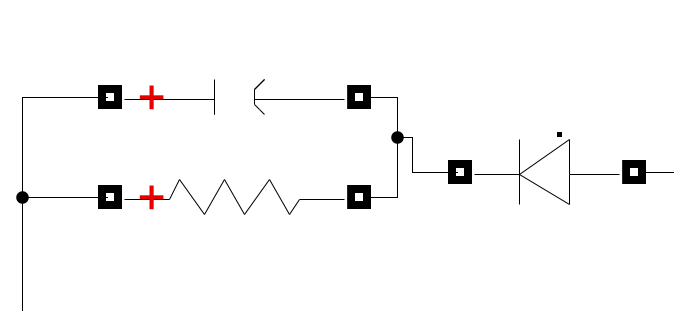
\includegraphics[width=0.4\textwidth]{Figs/snubberLay.PNG}
  \end{center}
  \vspace{-10pt}
  \caption{Snubber Layout}
  \label{Snubberlayout}
  \vspace{-10pt}
\end{wrapfigure}

When designing the RC snubber we can use an Application Note, in the application note, there is a snubber designed. We changed the R and C variables in order to adjust the solution into our problem. We have twice of voltage at the input and the current is twice. So, we used four times of R and two times of C. The values and the layout is in Figure \ref{Snubberlayout}:

$ R = 1250 \ohm$, $C=0.5 \micro F$


\subsection{Simulation of Non-ideal Case}

When we introduce all the non-idealities and run the simulation, the result is surprising. The output voltage waveform can be seen in Figure \ref{Output24non}

\begin{center}
\begin{figure}[H]
\centering
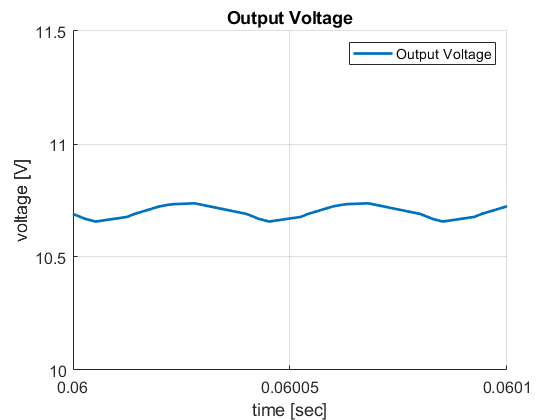
\includegraphics [width=12 cm, height= 8 cm]{output_voltage_non.png}
\caption{Output waveform of the forward converter 24V operation non-ideal}
\label{Output24non}
\end{figure}
\end{center}

We can see that due to the drops on the diodes, and the series parasitic resistances, the output voltage almost dropped to the $10.7V$. In order to compansate this value, we need to boost the duty cycle. We boost duty cycle to the 43.5\% for 24V operation.

\begin{center}
\begin{figure}[H]
\centering
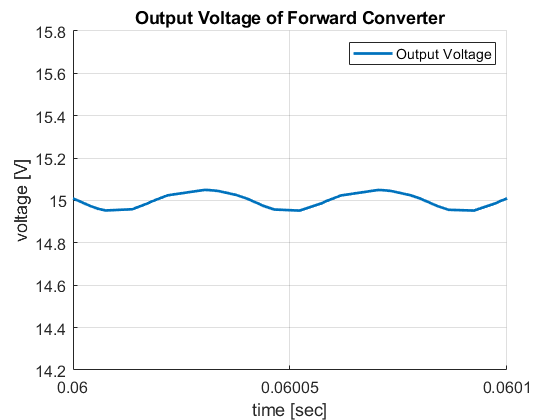
\includegraphics [width=12 cm, height= 8 cm]{output_voltage_com.png}
\caption{Output waveform of the forward converter 24V operation non-ideal}
\label{Output24com}
\end{figure}
\end{center}

\begin{figure}[H]
\centering
\begin{subfigure}{7 cm}
  \centering
  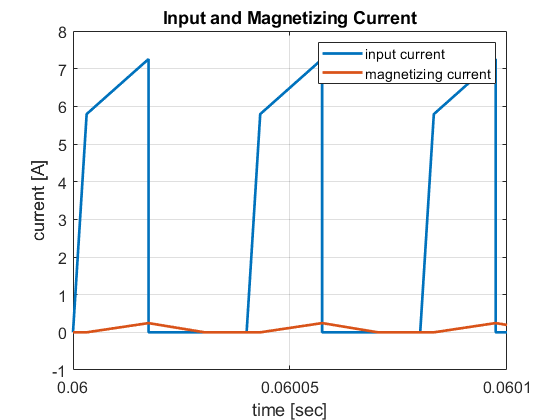
\includegraphics[width=7 cm]{Figs/input_current_24_com.png}
  \caption{Input and Magnetizing Current}
  \label{fig:input_current_24_com}
\end{subfigure}%
\begin{subfigure}{7 cm}
  \centering
  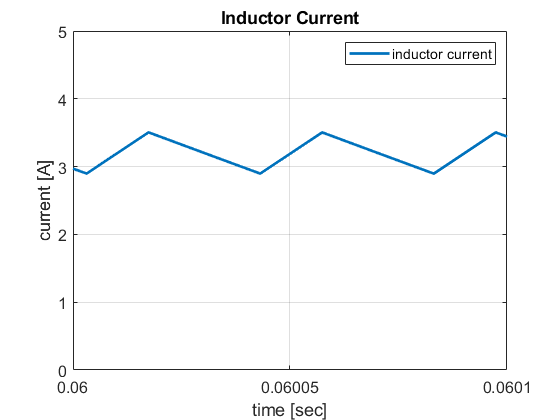
\includegraphics[width=7 cm]{Figs/inductor_current_com.png}
  \caption{Inductor Current}
  \label{fig:inductor_current_24_com}
\end{subfigure}
\caption{Forward converter input and inductor current under 24 non-ideal operation}
\label{fig:current_24}
\end{figure}

\begin{center}
\begin{figure}[H]
\centering
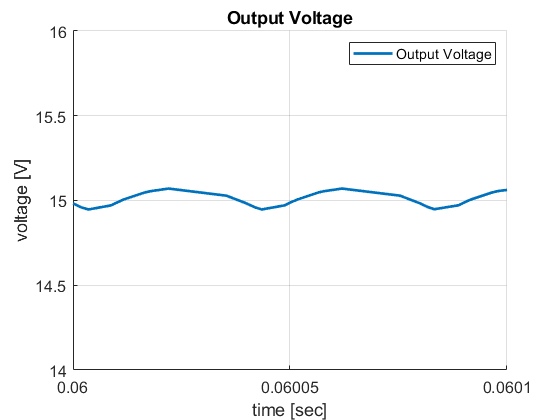
\includegraphics [width=12 cm, height= 8 cm]{output_voltage_non48.png}
\caption{Output waveform of the forward converter 48V non-ideal operation}
\label{Output48com}
\end{figure}
\end{center}

\begin{figure}[H]
\centering
\begin{subfigure}{7 cm}
  \centering
  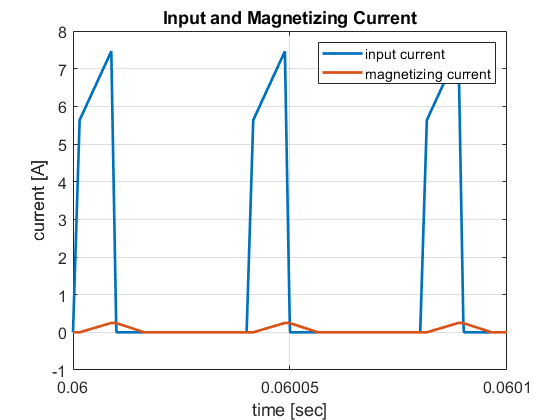
\includegraphics[width=7 cm]{Figs/input_current_non48.png}
  \caption{Input and Magnetizing Current}
  \label{fig:input_current_48_com}
\end{subfigure}%
\begin{subfigure}{7 cm}
  \centering
  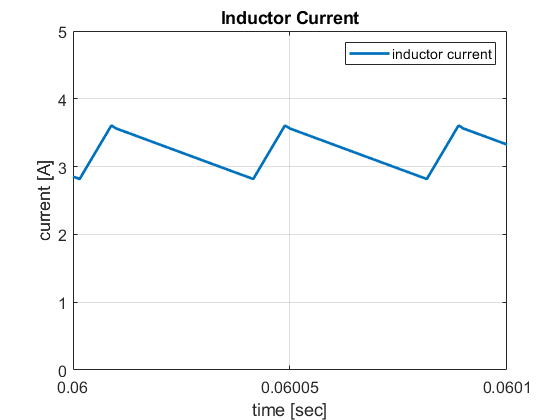
\includegraphics[width=7 cm]{Figs/inductor_current_non48.png}
  \caption{Inductor Current}
  \label{fig:inductor_current_48_com}
\end{subfigure}
\caption{Forward converter input and inductor current under 48V non-ideal operation}
\label{fig:current_24}
\end{figure}

The above simulations are for the non-ideal case with open-loop operation. Non-idealities drop the output voltage almost 2/3 of its value and decreases efficiency. Efficiency analysis will be done in the following parts.

In the ideal operations the duty cycles were calculated as: $D_{min} = 15.65\%$ and $D_{max} = 31.25\%$. However, in the non-ideal cases these values arised to higher values. So, it is very important to take non-idealities into account. This may result in inapplicable duty cycle values. Fortunately, our turn ratio decision $N=2$ is enough for non-ideal operation. Our non-ideal case duty cycles are:

$D_{min} = 22.05\%$, and $D_{max} = 43.5\%$

One of the most important parts is the snubber around the switch. We know that the leakage inductance of the transformer create high voltages around the switch and causes burn outs. We designed a snubber circuit and introduced it. The results of non-ideal switching with snubber is below:

\begin{figure}[H]
\centering
\begin{subfigure}{7 cm}
  \centering
  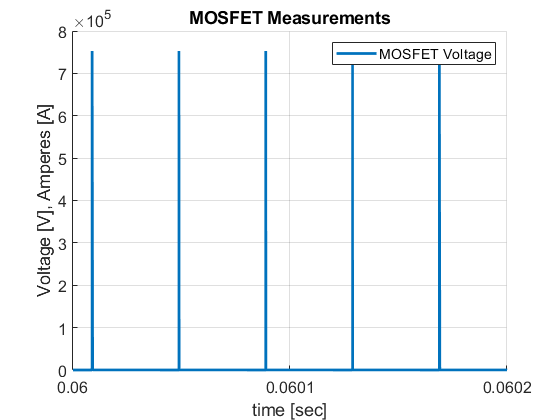
\includegraphics[width=7 cm]{Figs/nosnubber.png}
  \caption{MOSFET Voltage without Snubber}
  \label{fig:input_current_24_com}
\end{subfigure}%
\begin{subfigure}{7 cm}
  \centering
  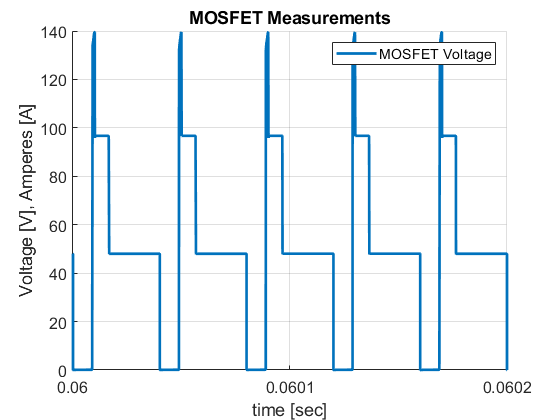
\includegraphics[width=7 cm]{Figs/snubber.png}
  \caption{MOSFET Voltage with Snubber}
  \label{fig:inductor_current_24_com}
\end{subfigure}
\caption{Snubber effect on the MOSFET operation with leakage inductance}
\label{fig:snubber}
\end{figure}

Since our MOSFET has a rated voltage of 150V, it is applicable. This snubber design is working.



\section{Transfer Function and Compansator Design}
\subsection{Transfer Function Derivation}

In the transfer function derivation, we are going to use averaging method.

In the forward converter below Figure \ref{forward1} we can observe the forward converter. Here, we are starting with defining the $x_1 = i_L$ and $x_2 = v_c$. These two states will be taken into account from now on.

\begin{center}
\begin{figure}[H]
\centering
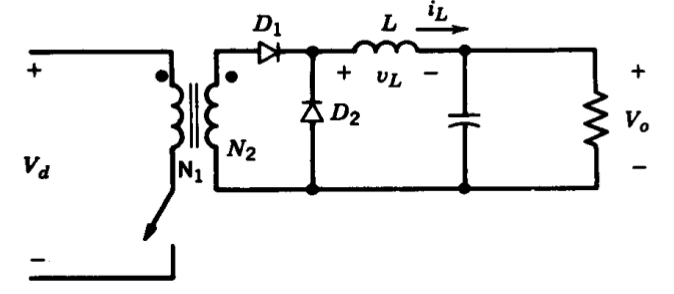
\includegraphics [width=12 cm, height= 6 cm]{forward.png}
\caption{Forward Converter Topology}
\label{forward1}
\end{figure}
\end{center}

When we use the averaging method. It is important to use the switch ON and switch OFF models of the converter. Below, we can observe these models in Fig. \ref{fig:switch}.

\begin{figure}[H]
\centering
\begin{subfigure}{7 cm}
  \centering
  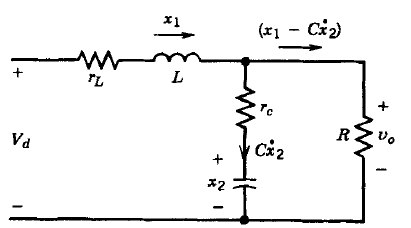
\includegraphics[width=7 cm]{Figs/switchON.PNG}
  \caption{Switch ON}
  \label{fig:input_current_48}
\end{subfigure}%
\begin{subfigure}{7 cm}
  \centering
  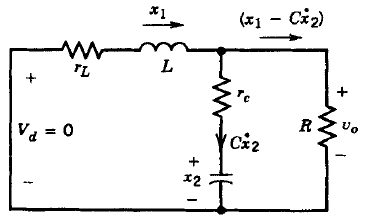
\includegraphics[width=7 cm]{Figs/switchOFF.PNG}
  \caption{Switch OFF}
  \label{fig:inductor_current_48}
\end{subfigure}
\caption{Forward converter averaging models switch on (a) and switch off (b)}
\label{fig:switch}
\end{figure}

In the first model, we can write that: assuming turn ratio is N.

\begin{equation}
    -NV_d + r_L i_L + L \Dot{i_L} + R(i_L - C\Dot{v_C}) = 0
\end{equation}

and 

\begin{equation}
    -v_c + C r_c \Dot{v_C} + R(i_L - C\Dot{v_c}) = 0
\end{equation}

Basically, when switch is on if we call this state space representation number 1, then it will have following structure:

\begin{equation}
\begin{bmatrix}
\Dot{i_L} \\ \Dot{v_C}
\end{bmatrix}
=
\begin{bmatrix}
 -\dfrac{Rr_c + Rr_L + r_C r_L}{L(R + r_C)} & -\dfrac{R}{L(R + r_C)} \\
 \dfrac{R}{C(R + r_C)} & -\dfrac{R}{L(R + r_C)} 
\end{bmatrix}
\begin{bmatrix}
i_L \\ v_C
\end{bmatrix}
+
\begin{bmatrix}
\dfrac{1}{L} \\ 0
\end{bmatrix}
NV_d
\end{equation}

Let us call this state space representation as

$$ \Dot{x} = A_1 x + B_1 u$$

When the switch is off, we can write following equations:
\begin{equation}
  r_L i_L + L \Dot{i_L} + R(i_L - C\Dot{v_C}) = 0  
\end{equation}
and

\begin{equation}
    -v_c + C r_c \Dot{v_C} + R(i_L - C\Dot{v_c}) = 0
\end{equation}

Switch is off, if we call this state space representation number 2, then it will have following structure:

\begin{equation}
\begin{bmatrix}
\Dot{i_L} \\ \Dot{v_C}
\end{bmatrix}
=
\begin{bmatrix}
 -\dfrac{Rr_c + Rr_L + r_C r_L}{L(R + r_C)} & -\dfrac{R}{L(R + r_C)} \\
 \dfrac{R}{C(R + r_C)} & -\dfrac{R}{C(R + r_C)} 
\end{bmatrix}
\begin{bmatrix}
i_L \\ v_C
\end{bmatrix}
\end{equation}

Let us call this state space representation as

$$ \Dot{x} = A_2 x$$

As we can easily see $A_1 = A_2$ and more importantly $B_2 = 0$. Therefore averaging is much easier in this topology. Now, we can say that

\begin{equation}
    A = A_1D + A_2(1-D) = A_1
\end{equation}
and

\begin{equation}
    B = B_1D
\end{equation}

Let's derive the output. If we are to define the output as $v_o$ then we can write that

\begin{equation}
    v_o = R(i_L - C\Dot{v_C})
\end{equation}

in state space form for both switch on and off cases

\begin{equation}
    v_o = \begin{bmatrix}
    \dfrac{R r_c}{R+r_C}i_L & \dfrac{R}{R+r_c}v_C
    \end{bmatrix}
\end{equation}

To simplify these state space representations, we will follow a simple approach. In our circuitry, $r_c = 3 m\ohm$, $r_L = 60 m\ohm$ where $R = 4.7 \ohm$. Starting from this point, apparently, we can assume that
\begin{equation}
R \gg (r_C + r_L)
\end{equation}

so A is simplified as:

\begin{equation}
    A = \begin{bmatrix}
 -\dfrac{r_c + r_L}{L} & -\dfrac{1}{L} \\
 \dfrac{1}{C} & -\dfrac{1}{CR} 
\end{bmatrix}
\end{equation}

B is simplified as:

\begin{equation}
    B = \begin{bmatrix} 
 \dfrac{1}{L} \\ 0 
\end{bmatrix}
D
\end{equation}

C is simplified as:

\begin{equation}
C =
    \begin{bmatrix}
    r_C & 1
    \end{bmatrix}
\end{equation}

Now, we need to introduce small signal perturbations to the system.
\begin{equation}
  d = D + \Tilde{d}  
\end{equation}
\begin{equation}
  v_o = V_o + \Tilde{v_o}  
\end{equation}
and 
\begin{equation}
  x = X + \Tilde{x}  
\end{equation}

Now the equation becomes:

\begin{equation}
    \Tilde{\Dot{x}} = A\Tilde{x} + B N V_d \Tilde{d}
\end{equation}

and 

\begin{equation}
    \Tilde{v_o} = C\Tilde{x}
\end{equation}

when we use the laplace transformation:

\begin{equation}
    \Tilde{x}(s) = [sI-A]^{-1}(B_1 V_d)\Tilde{d(s)}
\end{equation}

So, output to control transfer function can be written as:

\begin{equation}
\dfrac{\Tilde{v_o}(s)}{\Tilde{d}(s)} = C[sI-A]^{-1} B N V_d    
\end{equation}

\begin{equation}
   \dfrac{\Tilde{v_o}(s)}{\Tilde{d}(s)} = NV_d \dfrac{1 + sr_C C}{LC (s^2 + s (\dfrac{1}{RC} + \dfrac{(r_c + r_L)}{L}) + \dfrac{1}{LC}) }
\end{equation}

\subsection{Bode Plot of the Forward Converter}

Let's have a look at to the bode plot of the forward converter. In the ideal case where capacitor and inductor resistance does not exist, the transfer function can be simplified as:

\begin{equation}
   \dfrac{\Tilde{v_o}(s)}{\Tilde{d}(s)} = NV_d \dfrac{1}{LC (s^2 + s \dfrac{1}{RC} + \dfrac{1}{LC}) }
\end{equation}

When we obtain its bode plot using Matlab, the resulting graph is below Fig \ref{}

\begin{figure}[H]
\centering
\begin{subfigure}{7 cm}
  \centering
  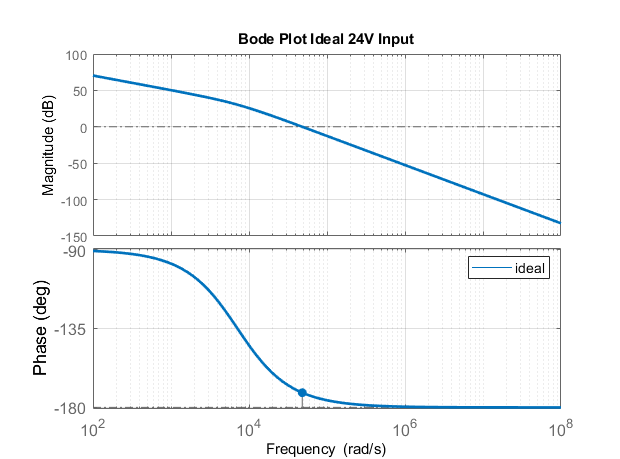
\includegraphics[width=7 cm]{Figs/bode_24_ideal.png}
  \caption{Ideal}
  \label{fig:bode_24}
\end{subfigure}%
\begin{subfigure}{7 cm}
  \centering
  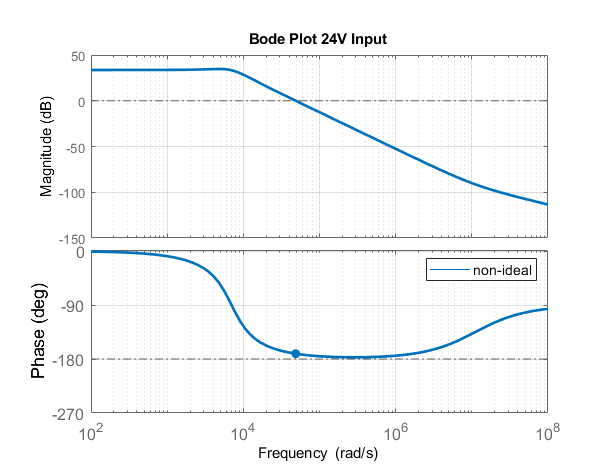
\includegraphics[width=7 cm]{Figs/bode_24_non.png}
  \caption{Non-ideal}
  \label{fig:bode_non_24}
\end{subfigure}
\caption{Bode plot with input 24V ideal (a) and non-ideal (b)}
\label{fig:bode24}
\end{figure}

\begin{figure}[H]
\centering
\begin{subfigure}{7 cm}
  \centering
  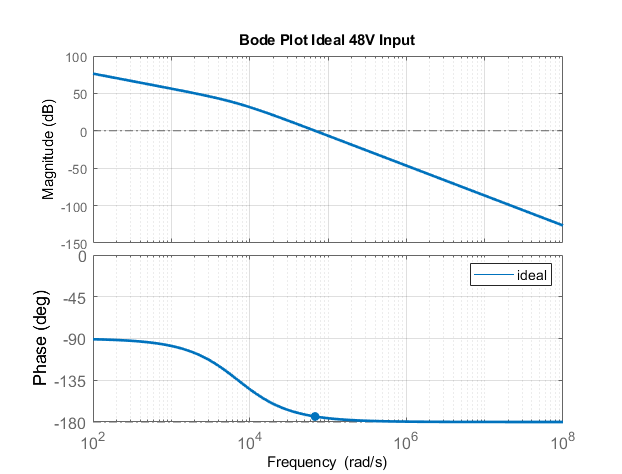
\includegraphics[width=7 cm]{Figs/bode_48_ideal.png}
  \caption{Ideal}
  \label{fig:bode_48}
\end{subfigure}%
\begin{subfigure}{7 cm}
  \centering
  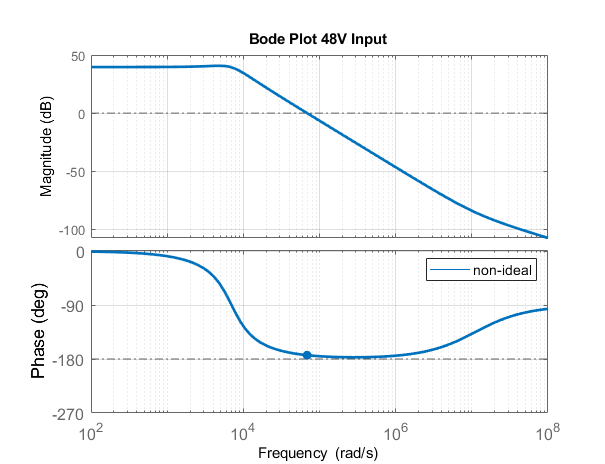
\includegraphics[width=7 cm]{Figs/bode_48_non.png}
  \caption{Non-ideal}
  \label{fig:bode_non_48}
\end{subfigure}
\caption{Bode plot with input 48V ideal (a) and non-ideal (b)}
\label{fig:bode48}
\end{figure}


At the worst case, the input is 48V. Below, we can observe the phase margin of 48V input bode plot with all non-idealities. Figure \ref{bode_big_48}

\begin{center}
\begin{figure}[H]
\centering
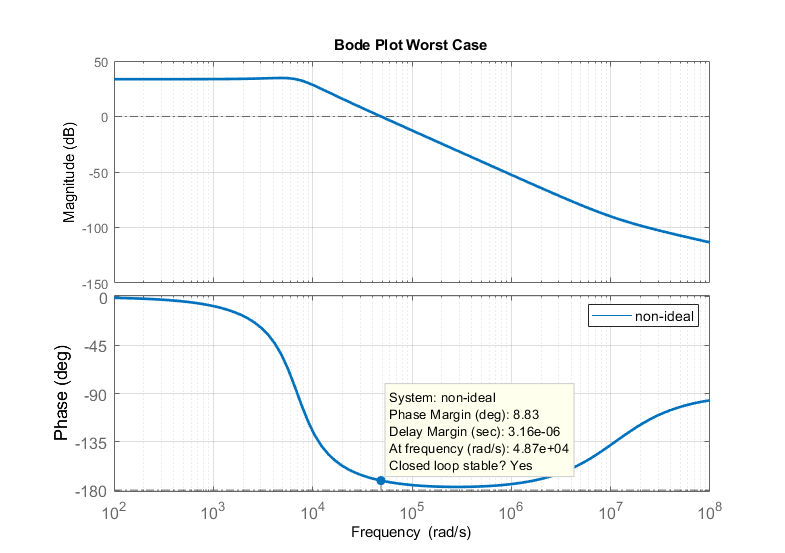
\includegraphics [width=14 cm]{bode_worst.png}
\caption{Bode plot of forward converter, worst case}
\label{bode_big_48}
\end{figure}
\end{center}

As we can follow, forward converter is a stable converter with a very small phase margin. Nevertheless, we need to design a compansator that will boost the phase of the converter so that we can operate in stable region with considerable speed. Now, we are going to design a compansator to make this system more stable. Also, we want to operate in constant output voltage!

\subsection{Compansator Design}

Basically, a forward converter and a boost converter have similar transfer functions. Its difference is that the input voltage reflects with a turn ratio, nonetheless, the rest is almost same. Therefore, we can apply a buck compansator for the forward converter, and make it work!


















\section{Efficiency and Thermal Analysis}
\subsection{Efficiency Analysis}

In the project, the converter is non-ideal, and there are losses expected to be. Now, analytically, one by one, we are going to cover the losses on the circuit.

\textbf{Capacitor ESR Losses}

Over the capacitor, the current that will flow is the amount of inductor current ripple. So, the average current over the capacitor is

\begin{equation}
    I_c = \dfrac{\Delta I_L T_s}{8} = 0.31A
\end{equation}

Easily, the loss on the ESR of the capacitor is:

\begin{equation}
    P_{esr,loss} = 0.31^2*0.003 = 0.3 mW
\end{equation}

It is a quite low value because we have chosen a ceramic capacitor.

\textbf{Inductor ESR Losses}

Over the inductor, the current flowing is 3.2A since output current is equal to inductor average current. 

\begin{equation}
    P_{L,loss} = 3.2^2*0.06 = 0.61W
\end{equation}

\textbf{Diode Losses}

Over the diodes, inductor current is flowing. So, easily:

\begin{equation}
    P_{D,loss} = 0.7 * 3.2 = 2.24W
\end{equation}

\textbf{MOSFET Loss}

Over the MOSFET, the loss at 10A current is given in the datasheet as 2.4W. We are going to use this value:

\begin{equation}
    P_{MOSFET} = 2.4W
\end{equation}


\textbf{Transformer Loss}

At the primary side:

\begin{equation}
    P_{pri} = 0.033 * 2^2 = 0.13W
\end{equation}

At the secondary side:

\begin{equation}
    P_{sec} = 3.2^2*0.045 = 0.46
\end{equation}

At the third winding

\begin{equation}
    P_{third} = 0.22^2 * 0.33 = 0.016W
\end{equation}

For the core loss, we should calculate the loss: 

Using the Magnetics R Material loss calculator, we have $124mW/cm^3$ loss in the core. Our core has a volume of $5.6*2 = 11.2 cm^3$

\begin{equation}
    P_{core} = 0.124 * 11.2 = 1.4W
\end{equation}

\textbf{Total Loss}

Total loss over the circuit is ignoring the leakage inductance:

\begin{equation}
    P_{total} = 0.003W + 0.61W + 2.24W + 2.4W + 0.13W + 0.46W + 0.016W + 1.4W = 7.3W
\end{equation}

\textbf{Efficiency}

Efficiency, ignoring the loss around the snubber:

\begin{equation}
    \eta = \dfrac{P_{out}}{P_{out} + P_{loss}} = \dfrac{48W}{48W+7.3W} = \dfrac{48W}{55.3W} = 86.7\%
\end{equation}

When, we simulate the circuit without using the snubber circuit the resultant efficiency is:

\begin{equation}
    \eta_{sim} = \dfrac{P_{out}}{P_{in}} = \dfrac{48W}{52.12W} = 92\% 
\end{equation}

However, this value does not include the core loss. When we analytically add the core loss on it!

\begin{equation}
    \eta_{total} = \dfrac{48W}{54.62W} = 87.8\% 
\end{equation}

Analytical calculations and simulation results are so similar!!

When we think of the snubber circuit, we can see that the average current around the snubber is:

\begin{equation}
    I_{snubber} = \dfrac{0.1}{2} = 0.05A
\end{equation}

\begin{equation}
    P_{snubber} = 0.05^2 * 1250 = 3.1W
\end{equation}

So, efficiency including the snubber is:

\begin{equation}
    \eta_{sn,total} = \dfrac{48W}{59W} = 81\%
\end{equation}

In the simulations, the efficiency simulated is 79\%. We can say that we have an efficiency of 80\% including the snubber circuit, leakage inductance, all ESR values and MOSFET, diode losses. This is a good efficiency for a forward converter.

\subsection{Thermal Analysis}

Losses on semiconductors are calculated in the previous subsection. By looking at their values and the thermal resistances of these components, we can have an idea if the temperature of these devices are within the operating range. Heatsinks can be used to cool them down. A heatsink suggestion will be made for the components in this section. 

\textbf{MOSFET}

Loss on MOSFET is calculated as 2.4 W. Thermal resistance is obtained from the datasheet. Two values are given based on the mounting specification of the device. If a copper pad is built under it the thermal resistance decreases significantly but that was not the practice in our design.

Normally, thermal resistance of the MOSFET is given as $113 \degree C \W$. Considering that the device can work properly up to 150 \degreeC, a heatsink is definitely required. Junction to case thermal resistance of the MOSFET is
$$R_{jc} = 1.1 \; \degree C /W$$
A heatsink as small as possible is chosen from DigiKey website. Datasheet can be found \href{https://www.digikey.com/product-detail/en/aavid-thermal-division-of-boyd-corporation/577102B00000G/HS106-ND/108319}{here}. It is cheap yet efficient. Thermal resistance value for the heatsink is 
$$R_{sink} = 25.9\; \degree C /W$$

Assuming that the ambient temperature is 25 C\degree, operating temperature for the MOSFET junction can be found as follows.
$$T_{op} = T_{amb} + P_{loss}*(R_{jc}+R_{sink}) \implies T_{op} = 25 + 2.4*27 \approx 90 \degree C $$

This value is reasonable for our device and operation can continue safely with no problems.

\textbf{Diodes}

From the datasheet, loss is obtained as 2.24 W on diodes. This value is very close to that of MOSFETs. Thermal resistance of diode is obtained from the datasheet as
$$R_{jc} = 3 \; \degree C /W$$
Same heatsink can be used for the diodes as well. Similar calculation yields nearly the same result.

$$T_{op} = T_{amb} + P_{loss}*(R_{jc}+R_{sink}) \implies T_{op} = 25 + 2.24*28.9 \approx 90 \degree C $$

We can say that with the suggested heatsink, semiconductors can operate at temperatures around 90\degreeC. Switching losses are not included in the calculations since switching frequency is relatively low, but the margin is high enough to compensate for them as well. 
\section{PCB Design}
A PCB design is done for the converter, as requested by the recent changes in the hardware project. An open source PCB design tool, KiCad is used for the design. Lots of schematic symbols and footprints created by the users were available online. The transformer model is created by the team only. 
\subsection{Feedback Controller}

To keep the voltage constant at 15V and to satisfy the line/load regulations, instead of the previously designed compensator, an analog IC controller is implemented on PCB. A very popular PWM controller IC for power supplies, \textbf{TL494} by \emph{Texas Instruments} is chosen. Additional features comes with it makes it a favorable choice and in this section, some of them that are implemented in our design are to be presented. 

Pin configuration of the module can be seen at Fig \ref{TL494_pin}
\begin{center}
\begin{figure}[H]
\centering
\includegraphics [width= 12 cm ]{TL494_pin.png}
\caption{Pin Configuration for TL494}
\label{TL494_pin}
\end{figure}
\end{center}

\textbf{Powering Up TL494}

To power up the module properly, a DC-DC converter is used. Input voltage to TL494 is set to 12 V. A DC-DC converter module by \emph{Artesyn Inc.}, ATA00B36S-L is used. It can supply 3W of power at 12 V from an input between 18-75 V. Our input voltage to the system falls in its operation range, therefore this module can be used with no problems. Datasheet regarding this module can be found \href{ https://www.artesyn.com/assets/ata_series_ds_01apr2015_79c25814fd.pdf}{here.} 

\textbf{Basic Wiring}
For the wirings described as of this subsection, the application note by the TI is used. [5]
TL494 is able to drive two switches together, but only one of the outputs is to be used in our project. First of all, the switching frequency of the module should be set. It is done by a simple RC circuit connected to pins 5 and 6. Internally it connects to the oscillator of the module and sets the frequency. Switch frequency is 25 kHz in our design. 
$$f_{switch} = \frac{1}{R_{T}C_{T}}$$

Standard values are chosen for the components and $f_{switch} \approx 25.9 kHz$ is achieved. 
$$R_{T} = 8.2 \;k\ohm$$
$$C_{T} = 4.7 \;nF$$

One of the error amplifiers in the module is for regulating the output voltage. The working principle is simple. Inverting input is fed by a constant voltage value from the voltage reference of the module. 2.5 V is chosen for this. And the non-inverting input is fed from the output voltage of the converter. A schematic is given in Fig \ref{TL494_volt}. 

\begin{center}
\begin{figure}[H]
\centering
\includegraphics [width= 10 cm ]{TL494_volt.png}
\caption{Output Voltage Regulation by TL494}
\label{TL494_volt}
\end{figure}
\end{center}

Output voltage of the converter is 15V, therefore the voltage divider resistances are chosen as follows.
$$R_1 = 10 \; k\ohm$$
$$R_2 = 2 \; k\ohm$$
Amplifier gain is increased to 101 with a simple feedback loop formed  between pins 2 and 3, inverting input and output of the amplifier respectively. Two resistors with ratings $51 k\ohm$ and $510 k\ohm$ are used to achieve this. 


\textbf{Current Limitation}

A second error amplifier is reserved for output current limitation. When the output current goes beyond the adjusted value, the gate signal to the converter is cut therefore a short-circuit protection is implemented by the control circuitry. 

Again, voltage reference output of the controller is fed to the inverting input of the current error amplifier. Voltage is set to 1V here. The current limit here is chosen as 5A in our application. Therefore, a really small resistor, referred to as $R_{13}$ in Fig \ref{TL494_current}, is connected in series with the load. In our application it is chosen as $\mathbf{0.2 \ohm}$.

\begin{center}
\begin{figure}[H]
\centering
\includegraphics [width= 10 cm ]{TL494_current.png}
\caption{Short Circuit Protection by TL494}
\label{TL494_current}
\end{figure}
\end{center}

\textbf{Soft Start Application}

There is only on switching element in our design, therefore the dead time application is not needed. Nevertheless, a soft starting mechanism is added. The wiring can be seen at Fig \ref{TL494_soft}. 

\begin{center}
\begin{figure}[H]
\centering
\includegraphics [width= 10 cm ]{TL494_soft.png}
\caption{Soft Start with TL494}
\label{TL494_soft}
\end{figure}
\end{center}

At the beginning of the regulation, $C_2$ capacitor charges through $R_6$ and by this way, the output pulse slowly increases till the control loop takes command. Considering $R_6$ is about one tenth of $R_T$ resistor, which corresponds to a $1 k\ohm$ resistance, the capacitor value can be calculated as follows. 50 cycles is chosen for the soft start time. 
$$C_{2} = \frac{Soft-start \: duration}{R_{6}} = \frac{40\micro s * 50}{1k\ohm} \approx 2.2 \micro F$$

\textbf{Gate Driver}

To ensure electrical isolation between input and output sections of the converter, an optocoupler is to be used to drive the switching element. Our choice for this element is \textbf{TLP250} by \emph{Toshiba}. It is a familiar IC for us, since it is used previously on the hardware project of EE463. A seperate power supply is needed to drive the gate driver, therefore there are two power input pin pairs to the converter : one for the main supply and for the gate driver. 
\subsection{Schematic}
A schematic is the first step to create a PCB. Kicad's "Eeschema" tool is used for this means. Generic symbols for diodes, inductors and such are used. Semiconductor symbols were available at the library. The symbol created for the three-winding transformer can be seen at Fig \ref{trafo}.

\begin{center}
\begin{figure}[H]
\centering
\includegraphics [width= 12 cm ]{trafo.png}
\caption{Schematic Symbol for Transformer in KiCad}
\label{trafo}
\end{figure}
\end{center}

Necessary wirings for TL494 are done as told in previous subsection. DC-DC Converter is added. Resulting schematic can be seen at Fig \ref{schematic}.

\begin{center}
\begin{figure}[H]
\centering
\includegraphics [width= 22 cm, angle=90 ]{schematic.png}
\caption{Converter Circuit Schematic in KiCad}
\label{schematic}
\end{figure}
\end{center}
\subsection{Footprints}
After the schematic is completed, components should be annotated and footprints should be assigned to each one of them. The packages are matched with each component chosen. The list  for the components used in the PCB Design and the corresponding footprint selections can be seen in Fig \ref{footprints}. 

\begin{center}
\begin{figure}[H]
\centering
\includegraphics [width= 12 cm ]{footprints.png}
\caption{Footprint List in KiCad}
\label{footprints}
\end{figure}
\end{center}

A footprint for the transformer was not readily built, since the transformer is to be designed by the team. Only the transformer's footprint is custom made. The dimensions of the chosen core is taken into consideration. 6 pads are formed for each ends of three windings. The resulting footprint can be seen in Fig \ref{trafo_foot}.

\begin{center}
\begin{figure}[H]
\centering
\includegraphics [width= 12 cm ]{trafo_foot.png}
\caption{Footprint for Transformer}
\label{trafo_foot}
\end{figure}
\end{center}

\subsection{PCB View}

After all these arrangements are made, the PCB design process can begin. There are some basic rules to that, although we are not so experienced in PCB design we tried to apply all we know. 

First of all, traces should not make perpendicular turns. This can cause serious EMI problems and should be avoided all the times. Second thing that is considered with utmost attention is the trace widths. In the converter, currents can reach up to 3-4 A during operation. A simple PCB trace width calculator is used to make sure that our design can carry such currents. For control parts, default trace width is used but at the input and output stages, trace widths are 22 and 32 mils, respectively. It is assumed that $2 oz/ft^2$ of copper will be used. 

In order to make connections easier and to use less vias, through hole resistors are used. This can be changed and compactness could be improved but overall, the design looked neat enough to us. Some components are flipped when necessity occured. 3-4 vias are used as well. 

The PCB View of the design can be seen in Fig \ref{pcb_view} at the next page. The copper filling for the back layer is also done but to make components and connections more visible, it is not given in the following representation. 

\begin{center}
\begin{figure}[H]
\centering
\includegraphics [width= 22 cm, angle=90 ]{pcb_view.png}
\caption{PCB Design in KiCad}
\label{pcb_view}
\end{figure}
\end{center}

\subsection{3-D View}
Transformer and connector models are absent but a 3-D View of the project is presented  below. 

\begin{center}
\begin{figure}[H]
\centering
\includegraphics [width= 12 cm ]{3d_front.png}
\caption{3-D View of the PCB, Top Layer}
\label{3d_front}
\end{figure}
\end{center}

\begin{center}
\begin{figure}[H]
\centering
\includegraphics [width= 12 cm ]{3d_back.png}
\caption{3-D View of the PCB, Bottom Layer}
\label{3d_back}
\end{figure}
\end{center}

\subsection{Arrangement for 1000 Pieces from PCBWay}

When the design is completed, Gerber files are obtained and the board is ready for production. As suggested in the GitHub page, PCBWay has been the choice for producing the board. Price for 5 pieces, which is the minimum number allowed is calculated as \textbf{\$ 63} and for 1000 pieces it is \textbf{\$ 1320}. 

Component prices are given in detail in the Bill of Materials (BOM) presented in the following pages. Overall manifacturing costs are calculated from BOMs.
\begin{itemize}
    \item One piece production cost : \textbf{\$52.43}
    \item 1000 piece production, cost per piece : \textbf{\$28.95}
\end{itemize}

It can be easily seen that mass production is more profitable. For each cases BOMs are presented in the Appendix. Original Excel files can be found at GitHub repository. 


\section{Conclusion}
In this project, our goal is to design a DC to DC converter. Our team has chosen forward converter configuration, \#FOR1, for the project. In this report, we introduced possible topologies and the rationale behind our selection. Then, we theoretically calculated the needs of the project and the components. A detailed component by component calculation has been provided. Moreover, simulations for each component have been done and introduced. With the light of the simulations, our selections and theoretical calculations have been supported. It is now possible to say that the design introduced in this simulation report is doable, and properly functional. In conclusion, EE464 lectures have prepared us academically. We strongly  believe that this project will enhance our understanding, and provide broader vision into power electronics area.
\newpage
\section{Appendix : Bill of Material Files}

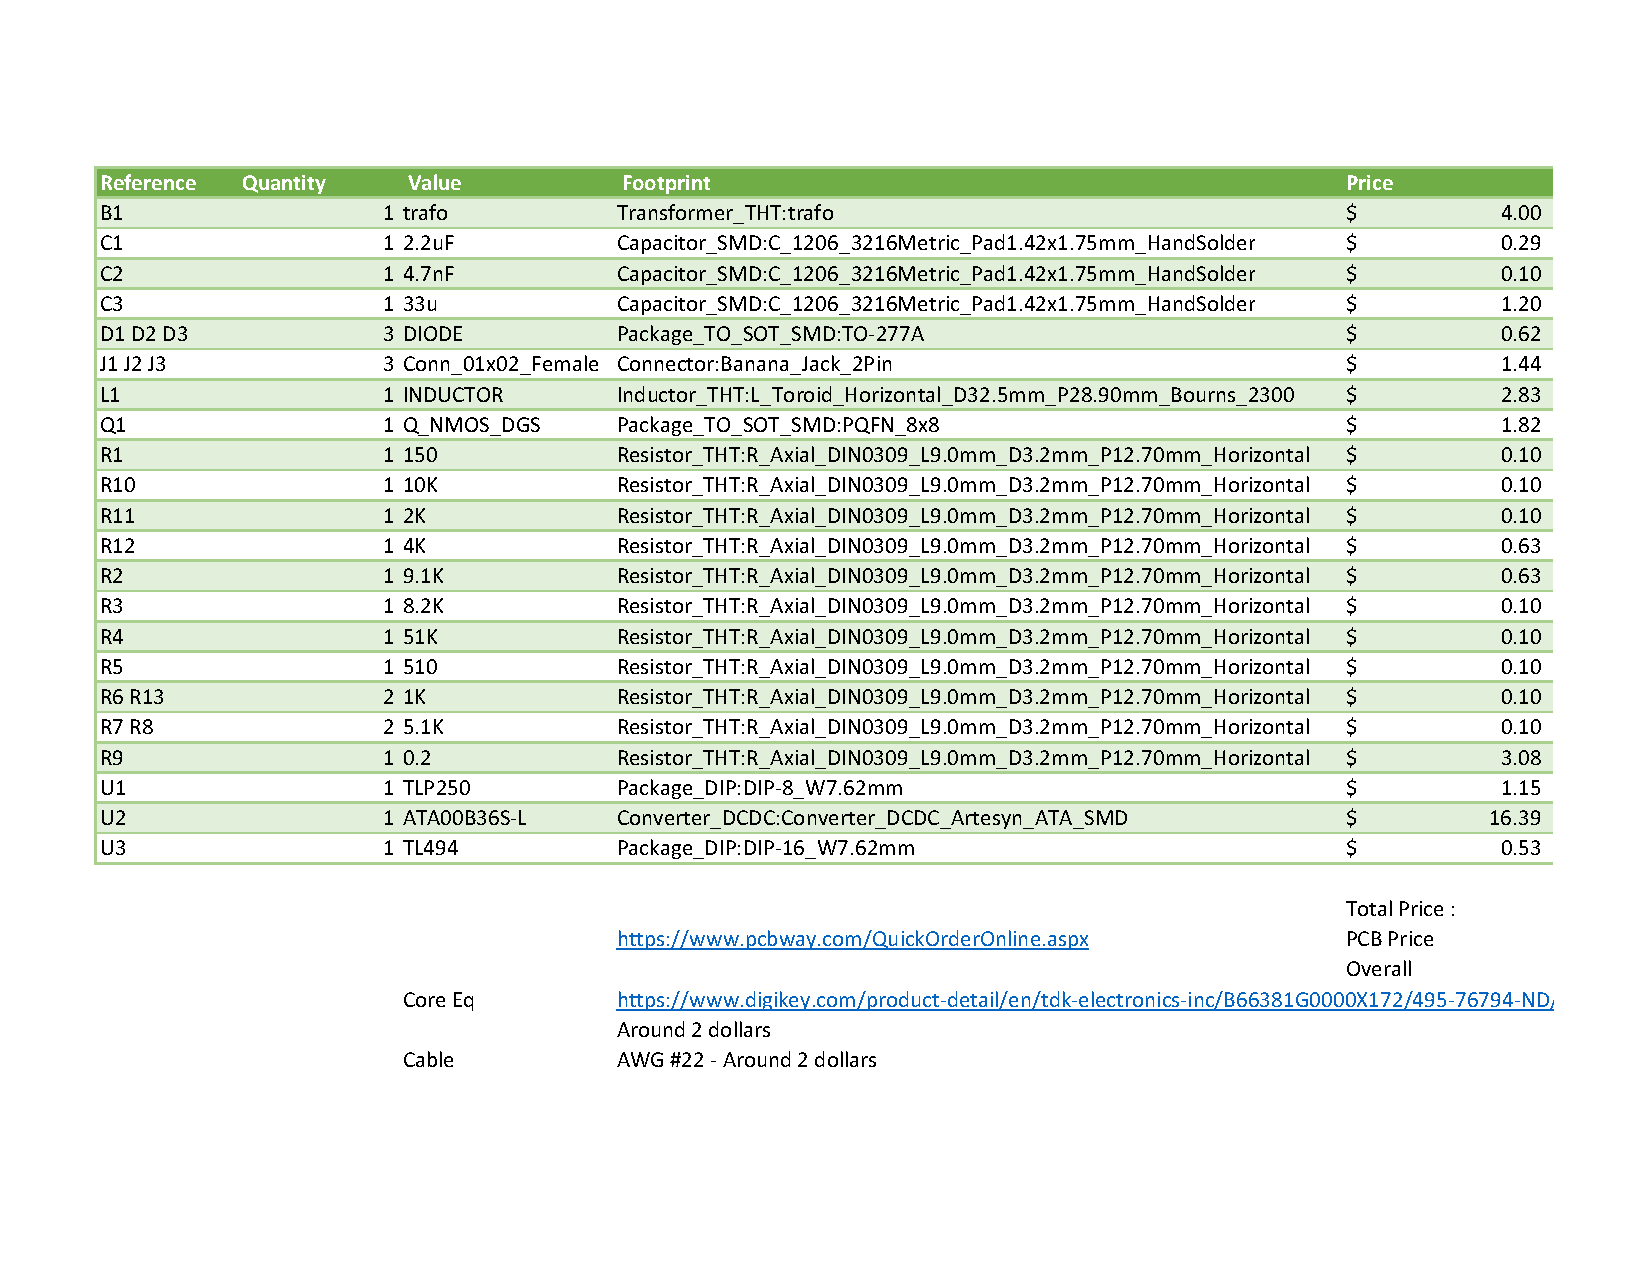
\includepdf[pages=-]{BOM.pdf}
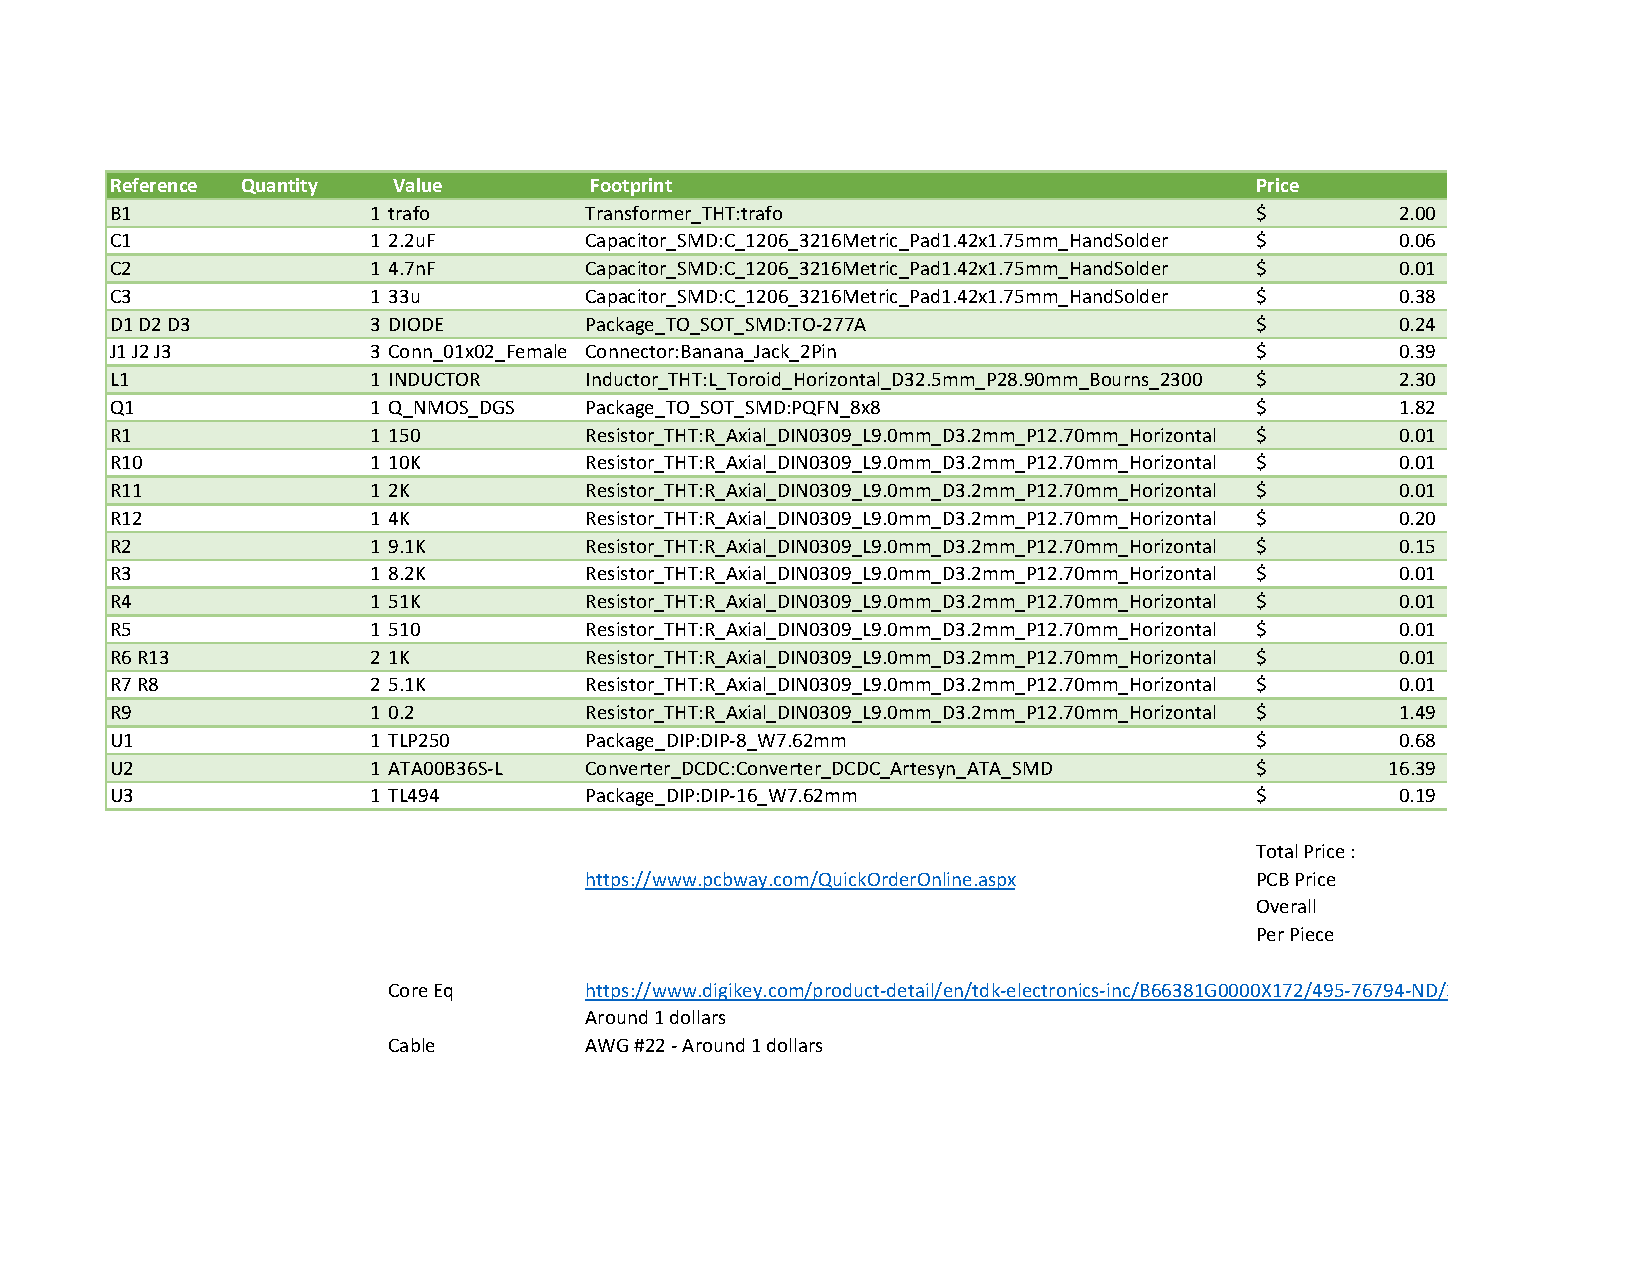
\includepdf[pages=-]{BOM_1000.pdf}

\begin{thebibliography}{9}
\bibitem{1} 
Transformer Design with Magnetics Ferrite Cores. [Online]. Available: https://www.mag-inc.com/Design/Design-Guides/Transformer-Design-with-Magnetics-Ferrite-Cores.

\bibitem{2}
"AN-776 20 Watt Simple Switcher Forward Converter", 2020. [Online]. Available: https://www.ti.com/lit/an/snva027a/snva027a.pdf?ts=1592752724490

\bibitem{3}
 N. Mohan, T. M. Undeland, and W. P. Robbins, Power Electronics: Converters, Applications, and Design. Hoboken, NJ: John Wiley \& Sons, 2003.

\bibitem{4}
"Compensator Design Procedure for Buck Converter with Voltage-Mode Error-Amplifier", Infineon.com, 2020. [Online]. Available: https://www.infineon.com/dgdl/an-1162.pdf?fileId=5546d462533600a40153559a8e17111a.

\bibitem{5}
Designing Switching Voltage Regulators With the TL494", 2020. [Online]. Available: https://www.ti.com/lit/an/slva001e/slva001e.pdf?ts=1592314978873

\end{thebibliography}
\end{document}